\newpage
\section*{Zielsetzung}
Bestimmung von Halbwertszeiten verschiedener Isotopen.
\section{Theorie}
Ist das Verhältnis von Neutronen- und Protonenzahl nicht innerhalb einer engen Grenze, so kann ein Atomkern mit einer bestimmenten Wahrscheinlichkeit in einen stabilen oder in einen instabilen Kern zerfallen. 
Eine typische emprirische Darstellung für die Wahrscheinlichkeit einer solchen Umwandlung drückt die Halbwertszeit $T$ aus, welche allerdings für verschiedene Zerfälle stark variiert.
Sie beschreibt den Zeitraum nachdem die Hälfte einer bestimmten Anzahl von instabilen Kernen Zerfallen ist.\\
Ursache für einen solchen Zerfall kann die Wechselwirkung mit einem Neutron sein.
\subsection{Neutronen als Ursprung von Kernreaktionen}
Wird ein Atomkern mit einem Neutrone beschossen, so führt die Absorption dessen zu einer Veränderung des Ursprungkerns $A$ zu einem Zwischenkern (bzw. Compoundkern) $A^*$.
Dieser Zwischenkern $\isotope{A}^*$ hat dem entsprechend eine höhere Energie als $\isotope{A}$, da sowohl die kinetische Energie des Netrons als auch dessen Bindungsenergie hinzukommt.
Durch die starke Wechselwirkung im Kern verteilt sich die Energie schnell im gesamten Kern und die Protonen und Neutronen beziehen schnell einen Erhöhten Energiezustand, diesen Prozess nennt man Aufheizung.
Durch die Energieverteilung als folge der Aufheizung ist es dem Kern nicht möglich direkt wieder ein Neutron abzugeben, daher wird falls das einfallende Neutron nur eine kleine kinetische Energie hatte nach nur $10^{-16}$ Sekunden ein $\gamma$ Photon emittiert um wieder in den Grundzustand zu gelangen.
\begin{equation}
    \isotope[m][z]{A} + \isotope[1][0]{n} \to \isotope[m+1][z]{A}^{*} \to \isotope[m+1][z]{A} + \gamma \nonumber
\end{equation}
Der entstandene Kern $\isotope[m+1][z]{A}$ ist oft nicht stabil aber hat eine deutlich längere Lebenszeit als der Zwischenkern $\isotope{A}^*$.
Der Kern $\isotope[m+1][z]{A}$ setzt sich aus folgenden Teilchen zusammen
\begin{equation}
    \isotope[m+1][z]{A} \to \isotope[m+1][z+1]{C} + e^- + E_{\text{kin}} + \bar{\nu_{\text{e}}} \label{eqn:Zerfall_A}
\end{equation}
Die Masse des Kerns ist dabei allerdings größer als die Summe der Teilchen in die er zerfällt.
Daher taucht beim Zerfall \ref{eqn:Zerfall_A} durch die Massendifferenz mit $\Delta E = mc^2$ die kinetische Energie $E_{\text{kin}}$ auf, die zu Teilen dem Elektron und dem Neutrino zukommt.

\subsection{Wirkungsquerschnitt?????}
Die Wahrscheinlichkeit dass ein Neutron von einem Kern eingefangen wird bezeichnet man als Wirkungsquerschnitt $\sigma$.
Der Wirkungsquerschnitt entspricht dabei der Kernfläche, bei der alle auftreffenden Neutronen eingefangen werden würden.\\  
Dabei ergibt sich der Wirkungsquerschnitt als 
\begin{align}
    \sigma = \frac{u}{nKd} && [\sigma] = 10^{-24} \text{cm}^2 = 1 \text{barn}
\end{align}
Mit den Neutronen $n$ die pro Sekunde auf die Folie treffen, der Anzahl $u$ der Einfänge, der Dicke $d$ der Folie und der Anzahl $K$ der Atome pro $\text{cm}^2$.
Außerdem ist $\sigma$ damit abhängig von den eintreffenden Neutronen.
Insbesondere lassen sich schnelle Neutronen für dessen De-Broglie-Wellenlänge (\ref{eqn:De-Broglie}) und dem Kernradius $R$ gilt $\lambda \ll R (≈10^{-12}cm) $ geometrisch betrachten.
\begin{equation}
     \lambda = \frac{h}{m_{\text{n}} v} \label{eqn:De-Broglie}
\end{equation}
Für die langsamen Neutronen ist die einfachere geometrische Betrachtung durch quantenmechanische Effekte nicht mehr möglich.
In der Quantenmechanik tritt Absorption nur auf, wenn gilt $E_{\text{n}} = \Delta E$ für die Energiedifferenz $\Delta E$ zweier Zustände des Kerns.
Nach den Physikern Breit und Wigner lässt sich damit der Wirkungsquerschnitt in Abhängigkeit der Neutronenergie berechnen.
\begin{equation}
    \sigma(E) = \sigma_0 \sqrt{\frac{E_{r_{\text{i}}}}{E}} \frac{\tilde{c}}{\left(E-E_{r_{\text{i}}}\right)^2 + \tilde{c}}
\end{equation}
Die Variablen $\tilde{c}$ und $\sigma_0$ sind hierbei Konstaten und $E_{r_i}$ repräsentiert den jeweiligen Energiezustand.
Wenn nun $E \ll E_{r_{\text{i}}}$ kann $\left(E-E_{r_{\text{i}}}\right)^2$ als konstant angesehen werden und es folgt ein umgekehrt proportionaler Zusammenhang zwischen dem Wirkungsquerschnitt und der Neutronengeschwindigkeit.
\begin{equation}
    \sigma(E) \propto \frac{1}{\sqrt{E}} \propto \frac{1}{v}
\end{equation}

\subsection{Erzeugung niedrigenergetischen Neutronen}
Um Neutronen zu erzeugen werden $\isotope[9]{Be}$-Kerne mit $\alpha$ Teilchen aus dem Zerfall von $\isotope[226]{Ra}$ beschossen.
\begin{equation}
    \isotope[9][4]{Be} + \isotope[4][2]{\alpha} \to \isotope[12][6]{C} + \isotope[1][0]{n}
\end{equation}
Um die kinetische Energie der Neutronen zu verringern müssen sie noch Abgebremst werden.
Die Abbremsung wird durch eine Materieschicht in der die Neutronen elastisch mit der Materie stoßen realisiert.
Als passenedes Element für die Neutronen stellt sich Wasserstoff heraus, 
daher wird die Neutronenquelle von Paraffin umgeben. So führt ein Stoß ziwschen ihnen und dem Neutron
zur einer Energieübertragung nach
\begin{equation}
    E_ü=E_0\frac{4Mm}{(M+m)^2}.
\end{equation}
$E_ü$ beschreibt dabei die maximal übertragende Energie und $M$ und $m$ die Masse der
Stoßpartner.\\
Nach mehrfachen Stößen erreicht die Energie des PAraffins die gleiche mittlere kitnetische Energie 
wie die Moleküle in der Umgebung (ca. $0,0025\si{eV},T=290\text{°K}$).
Die resultierenden Neutronen mit der mittleren Geschwindigkeit von $2,2\si{km/s}$ nennt
man thermische Neutronen.
\begin{figure}
    \centering
    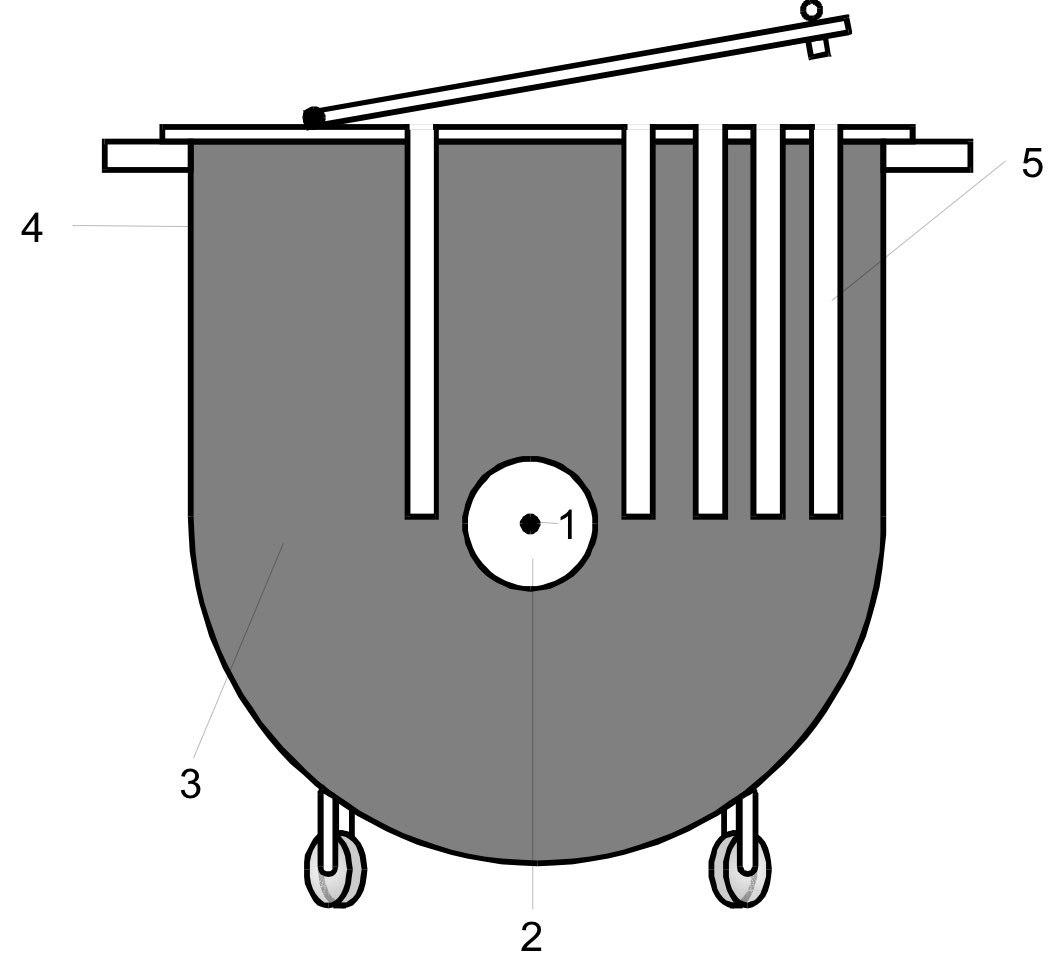
\includegraphics[width=0.4\textwidth]{bilder/Quelle.jpg}
    \caption{Dargestellt ist der Querschnitt der Quelle für thermische Neutronen.\cite[213]{anleitung}\\
    1 - Quelle schneller Elektronen\\
    2 - Bleiabschirmung\\
    3 - Paraffin\\
    4 - Stahlbehälter\\
    5 - Aktivierungsbohrung}
\end{figure}
\subsection{Halbwertszeit}
Die Anzahl N der noch nicht zuerfallenen Kerne zum Zeitpunkt $t$ kann durch
\begin{equation}
    N(t)=N_0\cdot e^{\lambda t},
\end{equation}
beschrieben werden. Dabei ist $N_0$ die Anzahl der Kerne zum Zeitpunkt $t=0$ und $\lambda$ 
die Zerfallskonstante. Für die Halbwertszeit $T$ gilt demnach
\begin{equation}
    \frac{1}{2}N_0=N_0\cdot e^{\lambda T},
\end{equation}
mit
\begin{equation}
    T=\text{ln}\left(\frac{2}{\lambda}\right).
\end{equation}

Da eine zuverlässige Messung von $N(t)$ einige Schwirigkeiten mitsich bringt, wird auf
die MEssung der zerfallenen Kerne in einem Zeitintervall $\Delta t$ zurückgegriffen.
So gilt
\begin{align}
    N_{\Delta t}(t)&=N(t)-N(t+\Delta t),\\
    N_{\Delta t}(t)&=N_0e^{-\lambda t}-N_0e^{-\lambda(t+\Delta t)}=N_0(1-e^{-\lambda\Delta t})e^{-\lambda t},\\
    \text{ln}(N_{\Delta t}(t))&=\text{ln}\left(N_0(1-e^{-\lambda\Delta t})\right)-\lambda t. \label{eqn:Zerfallsgesetz}
\end{align}

Das Zeitintervall $\Delta t$ muss dabei passend gewählt werden. Ist es zu klein
so folgen große statistische Fehler, ist es zu groß so folgen systematische Fehler für $\lambda$.
\label{subsec:halbwertszeit}